\documentclass[hidelinks,11pt,dvipsnames]{article}
% xcolor commonly causes option clashes, this fixes that
\PassOptionsToPackage{dvipsnames,table}{xcolor}
\usepackage[tmargin=1in, bmargin=1in, lmargin=0.8in, rmargin=1in]{geometry}

%%%%%%%%%%%%%%%%%%%%%%%%%%%%%%%%%%%%%%%%%%%%%%%%%%%%%%%%%%%%%%%%%%%%
%%% For inkscape-figures
%%% Assumes the following directory structure:
%%% master.tex
%%% figures/
%%%     figure1.pdf_tex
%%%     figure1.svg
%%%     figure1.pdf
%%%%%%%%%%%%%%%%%%%%%%%%%%%%%%%%%%%%%%%%%%%%%%%%%%%%%%%%%%%%%%%%%%%%
%\usepackage{import}
\usepackage{pdfpages}
\usepackage{transparent}

\newcommand{\incfig}[2][1]{%
    \def\svgwidth{#1\columnwidth}
    \import{./figures/}{#2.pdf_tex}
}

\pdfsuppresswarningpagegroup=1

% enable synctex for inverse search, whatever synctex is
\synctex=1
\usepackage{float,macrosabound,homework,theorem-env}
\usepackage{microtype}


% font stuff
\usepackage{sectsty}
\allsectionsfont{\sffamily}
\linespread{1.1}

% bibtex stuff
\usepackage[backend=biber,style=alphabetic,sorting=anyt]{biblatex}
\addbibresource{main.bib}

% colored text shortcuts
\newcommand{\blue}[1]{\color{MidnightBlue}{#1}}
\newcommand{\red}[1]{\textcolor{Mahogany}{#1}}
\newcommand{\green}[1]{\textcolor{ForestGreen}{#1}}


% use mathptmx pkg while using default mathcal font
\DeclareMathAlphabet{\mathcal}{OMS}{cmsy}{m}{n}

% fixes the positioning of subscripts in $$ $$
\renewcommand{\det}{\operatorname{det}}

\usetikzlibrary{positioning, arrows.meta}
\newcommand{\here}[2]{\tikz[remember picture]{\node[inner sep=0](#2){#1}}}

%%%%%%%%%%%%%%%%%%%%%%%%%%%%%%%%%%%%%%%%%%%%%%%%%%%%%%%%%%%%%%%%%%%%%
%%% Entry Counter
%%%%%%%%%%%%%%%%%%%%%%%%%%%%%%%%%%%%%%%%%%%%%%%%%%%%%%%%%%%%%%%%%%%%%
\newcounter{entry-counter}
\newcommand{\entry}[1]
{
	\addtocounter{entry-counter}{1}
    \tchap{Entry \arabic{entry-counter}}
	%\addcontentsline{toc}{section}{Entry \arabic{entry-counter}: #1}
	\vspace{-1.5em}
    \begin{center}
		\small \emph{Written: #1}
    \end{center}
}

\usepackage{titling}
\renewcommand\maketitlehooka{\null\mbox{}\vfill}
\renewcommand\maketitlehookd{\vfill\null}


\usepackage{capt-of}
\usepackage{tikz}
\usetikzlibrary{positioning,calc,intersections,through,backgrounds, shapes.geometric, decorations.markings,arrows}

\def\sset{\subseteq}
\def\iso{\cong}
\def\gend#1{\langle #1\rangle}

\newcommand{\rightoverleftarrow}{%
  \mathrel{\vcenter{\mathsurround0pt
    \ialign{##\crcr
      \noalign{\nointerlineskip}$\longrightarrow$\crcr
      \noalign{\nointerlineskip}$\longleftarrow$\crcr
    }%
  }}%
}

\newcommand\makesphere{} % just for safety
\def\makesphere(#1)(#2)[#3][#4]{%
  % Synopsis
  % \makesphere[draw options](center)(initial angle:final angle:radius)
  \shade[ball color = #3, opacity = #4] #1 circle (#2);
  \draw #1 circle (#2);
  \draw ($#1 - (#2, 0)$) arc (180:360:#2 and 3*#2/10);
  \draw[dashed] ($#1 + (#2, 0)$) arc (0:180:#2 and 3*#2/10);
}
% same thing as make sphere but places white background behind
\newcommand\altmakesphere{} % just for safety
\def\altmakesphere(#1)(#2)(#3)[#4][#5]{%
  % Synopsis
  % \make sphere[draw options](center)(initial angle:final angle:radius)
  \draw [fill=white!30] #1 circle (#2);
  \shade[ball color = #4, opacity = #5] #1 circle (#2);
  \draw #1 circle (#2);
  \draw ($#1 - (#2, 0)$) arc (180:360:#2 and 3*#2/10);
  \draw[dashed] ($#1 + (#2, 0)$) arc (0:180:#2 and 3*#2/10);
  \node at #1 {#3};
}

\begin{document}
% set section number to 1
% fixes theorem numbering without need to have a section title
\setcounter{section}{1}

\pagestyle{empty}
	\LARGE
\begin{center}
	Algebraic Topology Homework 10 \\
	\Large
	Isaac Martin \\
    Last compiled \today
\end{center}
\normalsize
\vspace{-4mm}
\hru

\tchap{Problems from 2.1}
\begin{homework}[e]
  \prob[\textsc{Exercise 16.}]$ $
  \begin{enumerate}[(a)]
    \item Show that $H_0(X,A) = 0$ if and only if $A$ meets each path-component of $X$.
    \item Show that $H_1(X,A) = 0$ if and only if $H_1(A) \to H_1(X)$ is surjective and each path-component of $X$ contains at most one path-component of $A$.
  \end{enumerate}
  \begin{prf}$ $
    \begin{enumerate}[(a)]
      \item Suppose first that $A$ meets all path components of $X$. To show $H_0(X,A) = 0$, it suffices to show that all relative $0$-cycles are equivalent to $0$-cycles in $A$. First, note that a $0$-simplex $\sigma:\Delta_0\to X$ is entirely determined by the image of the single point constituting $\Delta_0$, that is, there is a one-to-one correspondence between points of $X$ and $0$-simplicies. Denote the $0$-simplex sending the point in $\Delta_0$ to $x \in X$ by $\sigma_x$. Given a point $x\in X$, there exists a path $\gamma:[0,1]\to X$ such that $\gamma(1) = x$ and $\gamma(0) = a$ for some point $a \in A$, by the assumption that $A$ meets every path component of $X$. Such a path can be realized as a $1$-simplex via composition with an isomorphism $\Delta_1\xrightarrow{\sim} [0,1]$. Then $\delta(\gamma) = \sigma_x - \sigma_a$. As an element in $C_0(X,A)$, this is equivalent to $\sigma_x$ since $-\sigma_a \in C_0(A)$. But then $\sigma_x \in \img(\delta_1)$, and hence represents the trivial class in $H_0(X,A)$. Since $x$ was chosen arbitrarily, every $0$-simplex represents the trivial class in $H_0(X,A)$, so $H_0(X,A) = 0$.

        Now suppose that $H_0(X,A) = 0$. To show this implies $A$ meets every path component of $X$, we consider the long exact sequence
        \begin{align*}
          ... \to H_1(X,A) \xrightarrow{\partial} H_0(A) \xrightarrow{i_*} \xrightarrow H_0(X) \xrightarrow{j_*} H_0(X,A) \to 0.
        \end{align*}
        Recall that $i_*$ acts by sending a class $[\alpha] \in H_0(A)$ represented by a cycle to $[i(\alpha)] \in H_0(X)$. Since $H_0(X,A)$ is $0$, the map $i_*$ induced by the inclusion $A\hookrightarrow X$ must be surjective. This means for each $[\beta]\in H_0(X)$ there is some $[\alpha]\in H_0(A)$ such that $i(\alpha) = \beta$. This implies that $A$ has nontrivial intersection with the cycle $\beta$ in $X$. Taking $\beta$ to lie in a particular path component of $X$ gives the result, for as we have seen, $H_0(X)$ can be generated by choosing one cycle for each path component of $X$.

      \item Note first that each path component of $X$ contains at most one path component of $A$ if and only if $H_0(A) \xrightarrow{i_*} H_0(X)$ is injective. Recall that the free abelian group $H_0(A)$ can be generated by choosing a single cycle in each path component of $A$. If two path components $A_1$ and $A_2$ of $A$ are both intersect a path component  $X_1$ of $X$ nontrivially, then we can choose two cycles $a_1$ and $a_2$ corresponding in $A_1$ and $A_2$ respectively such that $i(a_1),i(a_2) \in X_1$. However, this means these are both cycles in a single path component of $X$, and hence represent the same element in $H_0(X)$.

        If instead $i_*:H_0(A)\to H_0(X)$ is not injective. Then we can find some element $[a] \neq 0 \in H_0(A)$ such that $i_*([a]) = 0$. Let $I$ be an index set for the path components $A_k$ of $A$ and $a_k$ be a cycle contained in $A_k$. Then we can find some $c_k \in \bZ$ such that only finitely many are nonzero and
        \begin{align*}
          [a] = \sum_{k\in I} c_k [a_k].
        \end{align*}
        Now applying $i_*$ gives $\sum_{k\in I} c_k i_*([a_k]) = i_*([a]) = 0$. If each $i_*([a_k])$ belonged to a separate path component of $X$, then the $c_k$ would necessarily be zero, but as this is not the case by the assumption that $[a] \neq 0$, at least two of the $i_*([a_k])$ lie in the same path component.

        \bigskip

        We now consider the same exact sequence as in part (a), but this time a little farther up:
        \begin{align*}
          ...\to H_2(X,A) \xrightarrow{\partial} H_1(A) \xrightarrow{i_*} H_1(X) \xrightarrow{j_*} H_1(X,A) \to H_0(A) \to ...
        \end{align*}
        Suppose first that $H_1(X,A) = 0$. By the exactness of this sequence, $H_1(A) \xrightarrow{i_*} H_1(X)$ is necessarily surjective. Likewise, further down the sequence, $H_1(X,A) = 0$ implies that $H_0(A) \to H_0(X)$ is injective, and hence by what we have already shown, each path component of $X$ contains at most one path component of $A$.

        Now suppose that $H_1(A)\to H_1(X)$ is surjective and each path component of $X$ contains at most one path component of $A$. The latter condition tells us that $H_0(A)\to H_0(X)$ is injective, and hence the relevant exact sequence reads
        \begin{align*}
          ... H_2(X,A) \to H_1(A) \xrightarrow{i_*} H_1(X) \xrightarrow{j_*} H_1(X,A) \xrightarrow{\partial} H_0(A) \xrightarrow{i_*} H_0(X) \to ...
        \end{align*}
        and so by problem 2.1.15 we have that $H_1(X,A)$ is necessarily $0$. To repeat a portion of the argument in this problem, the surjectivity of the first $i_*$ implies that the kernel of $j_*$ is all of $H_1(X)$, and so $\img j_* = 0$ in $H_1(X,A)$ and hence $\ker \partial = 0$. However, the injectivity of the latter $i_*$ implies that $\img \partial = 0$, so in particular $\ker \partial = H_1(X,A)$. This then implies $H_1(X,A) = 0$.
    \end{enumerate}
  \end{prf}
  \prob[\textsc{Exercise 17.}]$ $
  \begin{enumerate}[(a)]
    \item Compute the homology groups $H_n(X,A)$ when $X$ is $S^2$ or $S^1\times S^1$ and $A$ is a finite set of points in $X$.
    \item Compute the groups $H_n(X,A)$ and $H_n(X,B)$ for $X$ a closed orientable surface of genus two with $A$ and $B$ the circles shown. [What are $X/A$ and $X/B$?]
  \end{enumerate}
  \begin{prf}$ $
    \begin{enumerate}[(a)]
    \item Recall that if $A$ is a finite set of points, say $|A| = m$ for instance, then
      \begin{align*}
        H_n(A) =
        \begin{cases}
          \bZ^{\oplus m} & n = 0 \\
          0 & n > 0
        \end{cases}.
      \end{align*}
      We also know that
      \begin{align*}
        H_n(S^2) =
        \begin{cases}
          \bZ &n = 0,2 \\
          0 & \text{else}
        \end{cases}
        \textbuff{2em}{and}
        H_n(S^1\times S^1) =
        \begin{cases}
          \bZ & n = 0,2 \\
          \bZ^{\oplus 2} & n = 1 \\
          0 & \text{else}
        \end{cases}.
      \end{align*}
      Set $X = S^2$ and let $A \subseteq X$ be a finite subset consisting of $m$ points. Then the long exact sequence of the pair $(X,A)$ reads
      \begin{align*}
        ... 0 \to H_2(A) \xrightarrow{i_*} H_2(X) \xrightarrow{j_*} H_2(X,A) \xrightarrow{\partial} H_1(A) \to ...
      \end{align*}
      in index $2$. In all higher indices we have that $H_k(A) = H_k(X) = 0$, so this same exact sequence tells us $H_k(X,A) = 0$ whenever $k \geq 3$. Since $H_2(A) = H_1(A) = 0$, we get an isomorphism $H_2(X) \cong H_2(X,A)$. In the index $1$ position we have
      \begin{align*}
        ... 0 \xrightarrow{i_*} H_1(X) \xrightarrow{j_*} H_1(X,A) \xrightarrow{\partial} H_0(A) \xrightarrow{i_*} H_0(X) \to ...
      \end{align*}
      consider the rightmost map above. The group $H_0(A)$ is the free abelian group on $m$ generators $g_1,...,g_m$ and are all mapped by $i_*$ to the single generator $g$ of $H_0(X) = \bZ$, hence
      \begin{align*}
        \ker i_* = \left\{\sum_{j=1}^{m-1} a_jg_j ~-~ g \sum_{j=1}^{m-1}a_j \midd a_1,...,a_j \in \bZ\right\} \cong \bZ^{m-1}.
      \end{align*}
      This means $\img \partial = \ker i_* \cong \bZ^{m-1}$. The long exact sequence gives us a short exact sequence
      \begin{align*}
        0 \to H_1(X) \to H_1(X,A) \to \img \partial = \ker i_* \to 0,
      \end{align*}
      and because $\ker i_*$ is free, this short exact sequence splits giving us
      \begin{align*}
        H_1(X,A) \cong H_1(X) \oplus \ker i_* = 0 \oplus \bZ^{m-1}.
      \end{align*}
      For the final homology group, we have
      \begin{align*}
        ... \to H_0(A) \xrightarrow{i_*} H_0(X)\xrightarrow{j_*} H_0(X,A) \to 0.
      \end{align*}
      We have already seen that $H_0(A)\xrightarrow{i_*}H_0(X)$ is surjective, so $\ker (H_0(X) \to H_0(X,A)) = \img i_* = H_0(X)$ and implies that $j_*$ is the trivial map. However, exactness at $H_0(X,A)$ means that $j_*$ is surjective, and hence $H_0(X,A) = 0$. To summarize,
      \begin{align*}
        H_0(S^2,A) =
        \begin{cases}
          H_2(S^2) \cong \bZ & n = 2 \\
          H_1(S^2) \oplus \bZ^{m-1} \cong \bZ^{m-1} & n = 1 \\
          0 & \text{else}
        \end{cases}.
  \end{align*}

      Notice that nothing in our above argument relied on the fact that $X = S^2$. The only space-specific properties we needed were triviality of $H_n(X)$ for all $n \geq 3$ to get $H_n(X,A) = 0$ and the path connectedness of $X$ in order to see $i_*:H_0(A) \to H_0(X)$ was path connected. Both of these properties still hold for $X = S^1\times S^1$, so by the same arguments as above,
      \begin{align*}
        H_0(S^1\times S^1,A) =
        \begin{cases}
          H_2(S^1\times S^1) \cong \bZ & n = 2 \\
          H_1(S^1\times S^1) \oplus \bZ^{m-1} \cong \bZ^{m+1} & n = 1 \\
          0 & \text{else}
        \end{cases}.
      \end{align*}

    \item Let $X$ be the closed orientable surface of genus 2 and let $A$ and $B$ be the circles shown in figure \ref{fig:prob17-1}. Consider also tubular open neighborhoods $U$ of $A$ and $V$ of $B$, also shown in the figure.
    \begin{center}
      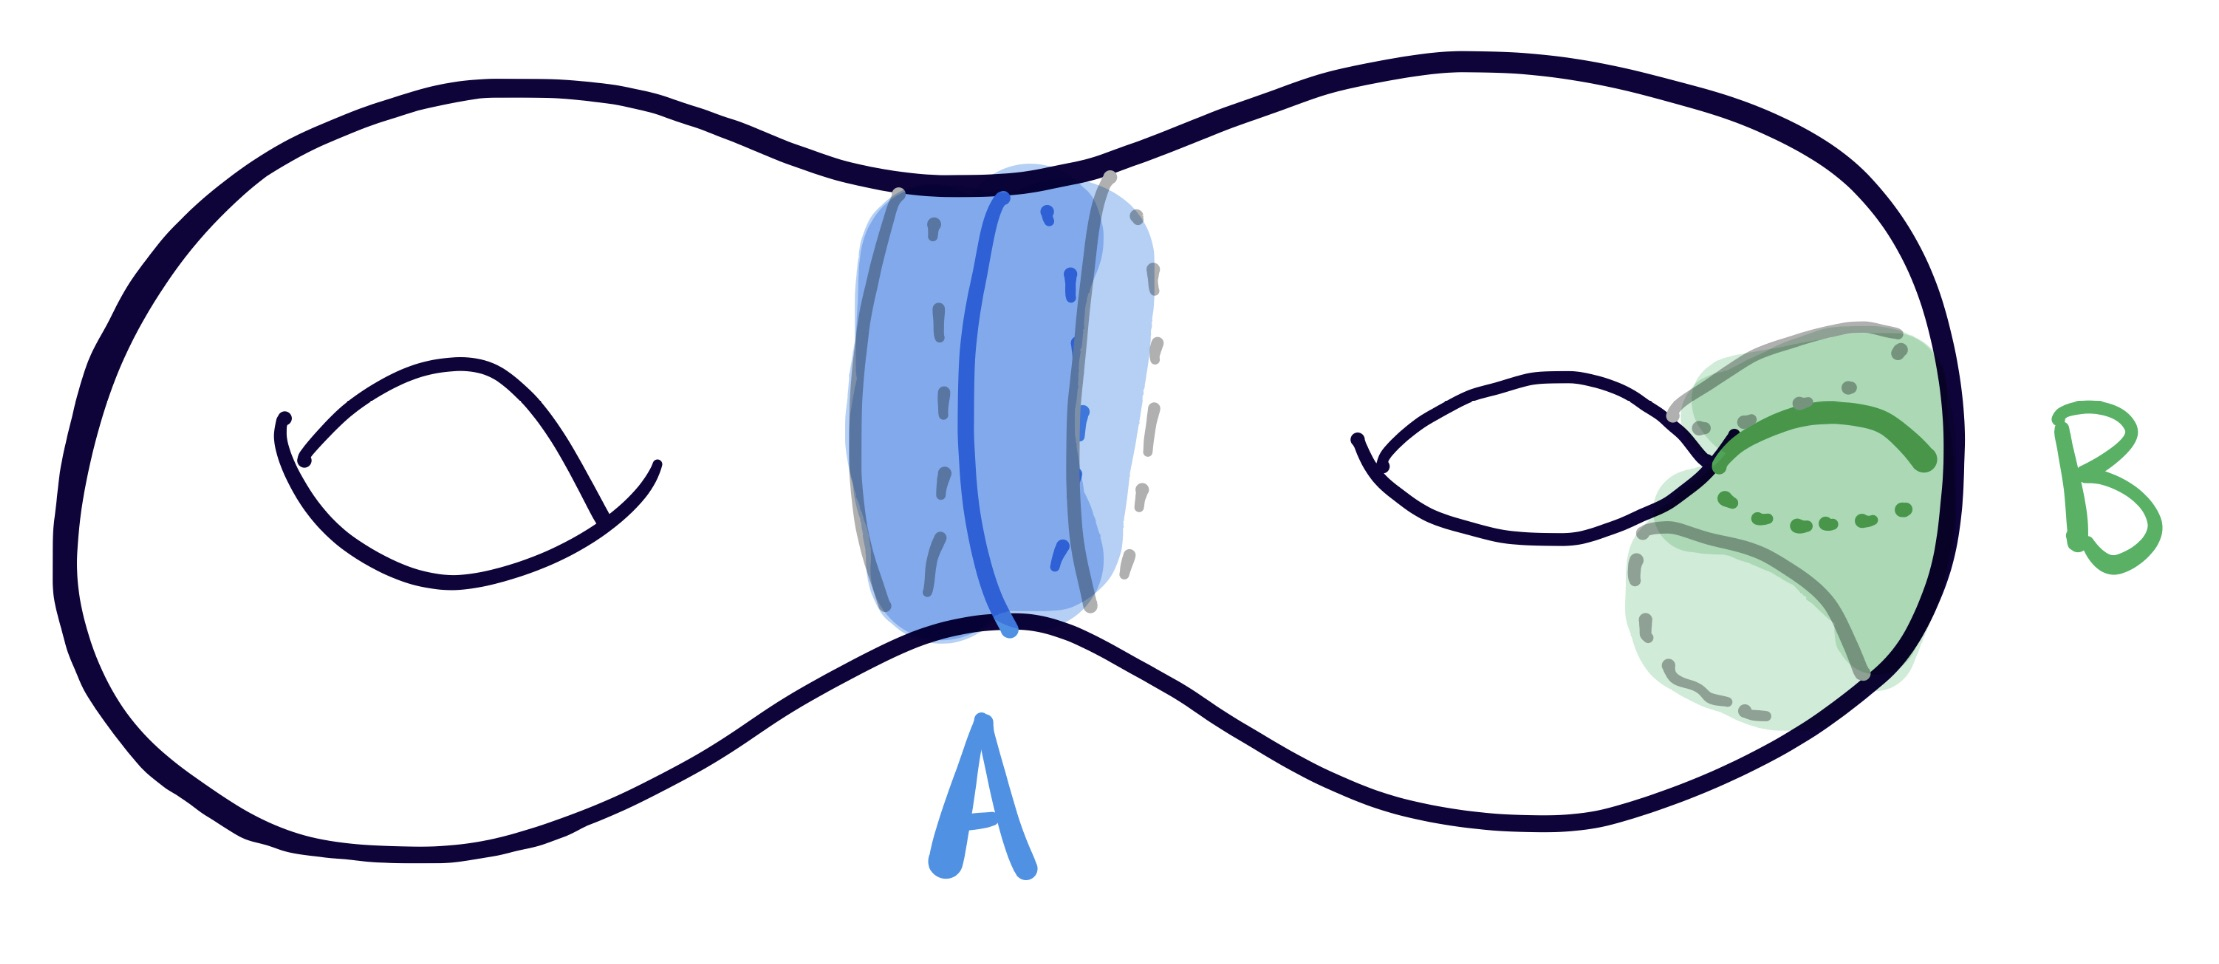
\includegraphics[width=12cm]{figures/hwk11-fig1.png}
      \captionof{figure}{Closed orientable surface of genus two with $A$ and $B$ circles}
      \label{fig:prob17-1}
    \end{center}
      The set $U$ deformation retracts onto $A$, so we have for any $k \in \bN$
      \begin{align*}
        H_k(X,A) \cong H_k(X,U) \cong H_k(X - A, U - A)
      \end{align*}
      where the last isomorphism follows from excision. The space $X - A$ has two connected components $X_1$ and $X_2$, each homeomorphic to two copies of the torus $T = S^1\times S^1$ each with a disk removed from the surface. The subset $U - A$ consists of a neighborhood around the boundary of each $X_i$ which deformation retracts to $\partial X_i$. Here we're lying a little bit -- $X_i$ doesn't contain its boundary -- but replacing $X_i$ with the closure $\ol{X_i}$ doesn't affect the homology groups. Regardless, since disjoint unions correspond to direct sums of homology groups,
      \begin{align*}
        H_k(X-A,U-A) \cong H_k(X_1,\partial X_1) \oplus H_k(X_2,\partial X_2).
      \end{align*}

      Consider the space $X_i$ a little more closely. This space is obtained from a torus $T$ by deleting a disk $D$. Let $x$ be a point in the interior of $D$ so that $D$ deformation retracts onto $x$. Then again by excision, we have
      \begin{align*}
        H_k(T,x) \cong H_k(T,D) \cong H_k(T - \{x\}, D - \{x\}) \cong H_k(X_1,\partial X_1).
      \end{align*}
      However, we are now in the scenario of part (a)  where our finite set consists now of only one element.Since $X_1 \cong X_2$, we can simply apply our previous results to get
      \begin{align*}
        H_n(X,A) \cong H_n(T,x) \oplus H_n(T,x)
        \begin{cases}
          \bZ^{2} & n = 2 \\
          \bZ^{4} & n = 1 \\
          0 & \text{else}
        \end{cases}.
      \end{align*}

      \bigskip

      Similarly, $V$ deformation retracts onto $B$, and applying excision gets us
      \begin{align*}
        H_k(X,B) \cong H_k(X,V) \cong H_k(X - B, V - B).
      \end{align*}
      The space $X - B$ is homeomorphic to a torus with two disjoint disks $D_1$ and $D_2$ removed:
    \begin{center}
      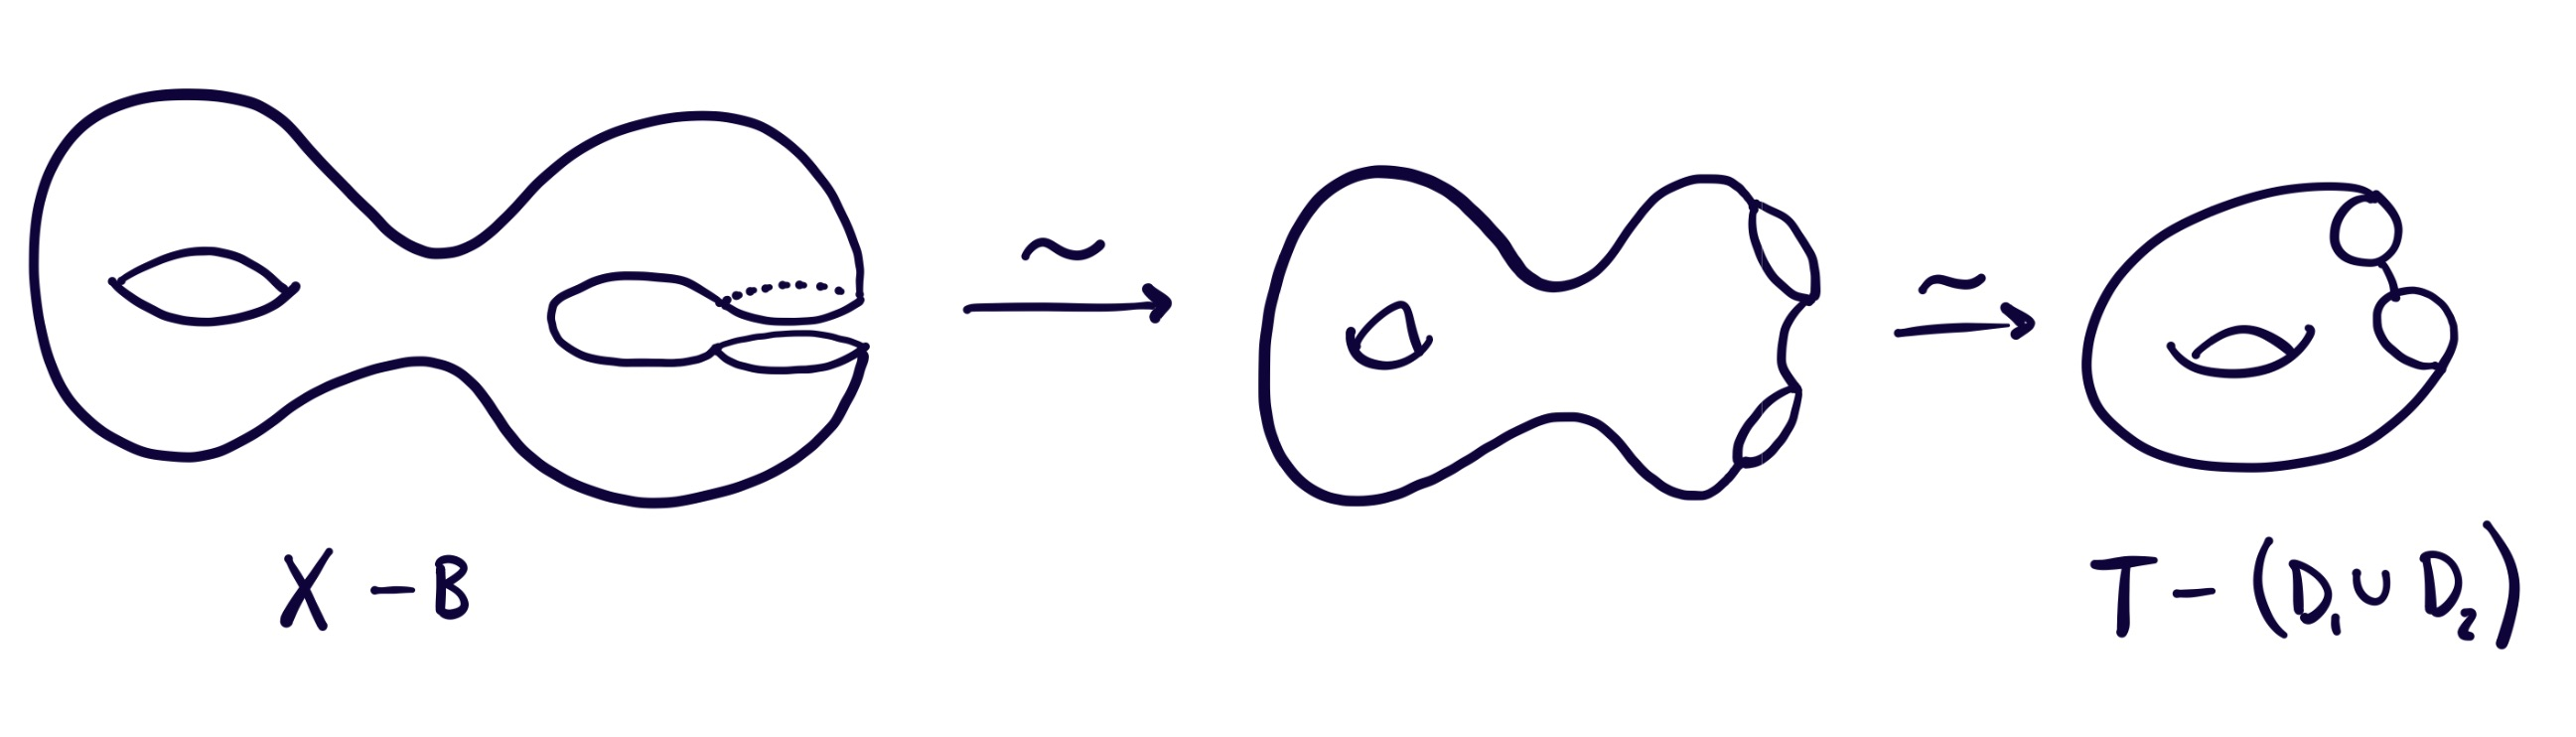
\includegraphics[width=12cm]{figures/hwk11-fig2.png}
      \captionof{figure}{$X - B$ is homeomorphic to $T - (D_1 \cup D_2)$}
      \label{fig:prob17-2}
    \end{center}
    Now choose $x_1 \in D_1$ and $x_2 \in D_2$. By applying an excision argument as before, we get that
    \begin{align*}
      H_k(T,\{x_1,x_2\}) \cong H_k(T - (D_1 \cup D_2), D_{1}\cup D_2 - \{x_1,x_2\}) \cong H_k(X - B, V - B).
    \end{align*}
    The rightmost homology group is again something we know from part (a), this time with $m = 2$, and so
    \begin{align*}
      H_n(X,B) \cong
      \begin{cases}
        \bZ & n = 2 \\
        \bZ^{3} & n = 1 \\
        0 & \text{else}
      \end{cases}.
    \end{align*}
    \end{enumerate}
  \end{prf}
  \prob[\textsc{Exercise 27.}] Let $f:(X,A)\to (Y,B)$ be a map such that both $f:X\to Y$ and the restriction $f:A\to B$ are homotopy equivalences.
  \begin{enumerate}[(a)]
    \item Show that $f_*:H_n(X,A)\to H_n(Y,B)$ is an isomorphism for all $n$.
    \item For the case of the inclusion $f:(D^n,S^{n-1}) \hookrightarrow (D^n,D^n - \{0\})$, show that $f$ is not a homotopy equivalence of pairs -- there is no $g:(D^n,D^n - \{0\})\to (D^n,S^{n-1})$ such that $fg $ and $gf$ are homotopic to the identity through maps of pairs. [Observe that a homotopy equivalence of pairs $(X,A) \to (Y,B)$ is also a homo copy equivalence for the pairs obtained by replacing $A$ and $B$ by their closures.]
  \end{enumerate}
  \begin{prf}$ $
    \begin{enumerate}[(a)]
      \item As noted by Prof. Allcock, this is a standard application of the five lemma. We have the following diagram:
        \begin{center}
          \begin{tikzcd}
            H_{n+1}(A) \arrow[r]\arrow[d,"f_*"]& H_{n+1}(X) \arrow[r]\arrow[d,"f_*"]& H_{n+1}(X,A) \arrow[r]\arrow[d,"f_*"]& H_n(A) \arrow[r]\arrow[d,"f_*"]& H_n(X)\arrow[d,"f_*"] \\
            H_{n+1}(B) \arrow[r]& H_{n+1}(Y) \arrow[r]&H_{n+1}(Y,B) \arrow[r]& H_{n}(B) \arrow[r]&H_{n}(Y)
          \end{tikzcd}
        \end{center}
        whose rows are exact due to the exactness of the long exact sequence of pairs whence the diagram arises. Since homotopy equivalences induce isomorphisms on absolute homology, the five lemma implies that the middle vertical map must also be an isomorphism. That's all there is to it, really.

      \item We argue by contradiction, and rather than $S^{n-1}$ we write $\partial D^n$. Suppose we have a map $g:(D^n,D^n \setminus \{0\})\to (D^n,\partial D^n)$ such that $gf$ is homotopic as a map of pairs to $\id_{(D^n,\partial D^n)}$. If $x \in D^{n}\setminus \{0\}$, then $g(tx) \in \partial D^n$ for all $t \in (0,1]$ and hence
        \begin{align*}
          g(0) = \lim_{x\to t^+} g(tx) \in \partial D^n
        \end{align*}
        by the continuity of $g$. This implies that $g(D^n) \subseteq \partial D^n$, so we may regard $g$ as a map $g:D^n \to \partial D^n$. Because $gf \simeq \id_{(\partial D, \partial D^n)}$ and $f$ is the inclusion, we have that $gf|_{\partial D^n} = g|_{\partial D^n} \simeq \id_{\partial D^n}$. This means that for every $k\geq 0$ we get a commutative diagram
        \begin{center}
          \begin{tikzcd}
            \tilH_{k}(\partial D^n) \arrow[r,"f_*"]\arrow[rd,"\id"] & \tilH_k(D^n) = 0 \arrow[d,"g_* = 0"] \\
                                                                                   & \tilH_k(\partial D^n)
          \end{tikzcd}
        \end{center}
        In particular, when $k = n-1$, we get $\tilH_k(\partial D^n)\cong \bZ$, in which case the diagram demands that $g_*f_* = \id$, which is impossible since $\tilH_k(D^n) = 0 \implies g_* = 0$. Hence we have our contradiction.
    \end{enumerate}
  \end{prf}
\end{homework}
\tchap{Problems from 3.3}
\begin{homework}[e]
  \prob[\textsc{Exercise 3.}] Show that every covering space of an orientable manifolds is an orientable manifold.
  \begin{prf}
    Let $M$ be an orientable manifold and let $p:\tilM\to M$ be a covering space of $M$. It is clear that $\tilM$ is a manifold -- it is locally homeomorphic to $M$ which is locally homeomorphic to $\bR^n$ -- so we need only show that $\tilM$ is orientable. Recall that by the definition of an orientation we have a function $\mu:M\to \{\pm 1\}$ which satisfies the local consistency condition:
    \begin{center}
      For all $x \in M$, there is some open ball $B \cong D^n \subseteq \bR^n$ of $x$ and $\mu_B$ a generator of $H_n(M, M - B)\cong \bZ$ such that for all $y \in B$ the local orientation $\mu_y$ is the image of $\mu_B$ under the natural isomorphism $H_n(M,M-B)\to H_n(M,M - y)$.
    \end{center}
    We show that the map $\mu \circ p$ is an orientation function for $\tilM$. To see this, fix an $x \in M$ and a $B$ as above. Let $U \subset \tilM$ be an open set mapped homeomorphically to $B$ by $p$ and $\tilx \in U$ be the unique preimage of $x$ in $U$. For any $\tily \in U$, we then have the following commutative diagram where all maps are isomorphisms:
    \begin{center}
      \begin{tikzcd}
        H_n(\tilM, \tilM - U) \arrow[d,"p_*"] \arrow[r,"\alpha"] & H_n(\tilM,\tilM - \tily)\arrow[d,"p_*"] \\
        H_n(M,M - B) \arrow[r,"\beta"] & H_n(M, M - p(\tily)),
      \end{tikzcd}
    \end{center}
    where the horizontal maps are the natural ones. If we define $\hat{\mu} = \mu\circ p$ then $\hat{\mu}_{\tily}$ is a local orientation at $\tily$. Let $\mu_U$ be the unique preimage of $\mu_B$ under $p_*$. Then by the commutativity of the diagram,
    \begin{align*}
      p_*(\alpha(\mu_U)) = \beta(p_*(\mu_U)) = \beta(\mu_U) = \mu_{p(\tily)},
    \end{align*}
    and since $p_*$ is an isomorphism, $\alpha(\mu_U) = \hat{\mu}_{\tily}$. Hence $\hat{\mu}$ is an orientation $\tilM$.
  \end{prf}
  \prob[\textsc{Exercise 4.}] Given a covering space action of a group $G$ on an orientable manifold $M$ by orientation-preserving homeomorphisms, show that $M/G$ is also orientable.
  \begin{prf}
    Suppose the group $G$ acting on $M$ via orientation preserving homeomorphisms is a covering space action and denote by $\pi:M\to M/G$ the projection map, recalling that this map is open. Because $G$ acts via a covering space action, $\pi$ is a local homeomorphism. To state this in the way most useful to us, this implies that for each $\olx \in M/G$ we can find some open neighborhood $\olU$ of $\olx$ such that there is some neighborhood $U$ of $x\in M$, a lift of $\olx$, for which $\pi|_U:U\to \olU$ is a homeomorphism. Now choose some open ball $B$ around $x$ such that $B$ satisfies the local consistency condition. By choosing $B$ to be small enough, we can ensure its closure is contained in $U$, and can thus be used in excision. We then have the following commutative diagram:
    \begin{center}
      \begin{tikzcd}
        H_n(M, M - x) \arrow[r,"\pi_*"]& H_n(M/G, M/G - \olx) \\
        H_n(M,M - B) \arrow[u] \arrow[r,"\pi_*"]& H_n(M/G,M/G - \pi(B)) \arrow[u]\\
        H_n(U,U - B) \arrow[u]\arrow[r,"\pi_*"]& H_n(\pi(U),\pi(U) - \pi(B)) \arrow[u]
      \end{tikzcd}
    \end{center}
    where the all vertical maps are isomorphisms, the lower ones arising from excision. Now consider a choice of generator $\mu_B$ which reproduces the local choice of generator $\mu_x$ at $x$. Then by commutativity, $\mu_{\pi(B)}$ is a choice of generator whose image in $H_n(M/G,M/G - \olx)$ is $\mu_{\olx}$. We are not quite done, as this may depend on the choice of lift $x$ of $\olx$. However, since the $G$ action is orientation preserving, any other choice $gx$ of representative for $\olx$ and $gB$ for neighborhood of $gx$ will still satisfy the local consistency condition, so we are done.
  \end{prf}
  \prob[\textsc{Exercise 7.}] For a map $f:M\to N$ between connected closed orientable $n$-manifolds with fundamental classes $[M]$ $[N]$, the degree of $f$ is defined to be the integer $d$ such that $f_*([M]) = d[N]$, so the sign of the degree depends on the choice of fundamental classes. Show that for any connected closed orientable $n$-manifold $M$ there is a degree $1$ map $M\to S^n$.
  \begin{prf}
    This argument is extraordinarily quick if we use the result of exercise 8. Luckily, exercise 8 can be proven without the result of exercise 7.

    Fix any open ball $B \subseteq M$. The quotient space $M/(M-B)$ obtained by collapsing the complement of $B$ to a point is then homeomorphic to $S^n$. Indeed, the quotient map $\pi:M \to M/(M-B)$ can be seen as the construction of $S^n$ as a cell complex: it maps $B$ homeomorphically to a copy of itself in $M/(M-B)$ and send the boundary of $B$ to the point corresponding to the newly collapsed complement of $B$. 
    
    By composing $\pi$ with the homeomorphism $M/(M - B)\cong S^n$ we obtain a map $f:M\to S^n$. Let $x = f(M/B)\in S^n$. Then $S^n - x$ is an $n$-ball and $f^{-1}(S^n - x) = B$. The restriction $f|_{B}$ is orientation preserving since the orientation of $M/(M - B)$ arises from $M$, and hence by exercise 8 $\deg f = 1$.
    \begin{center}
      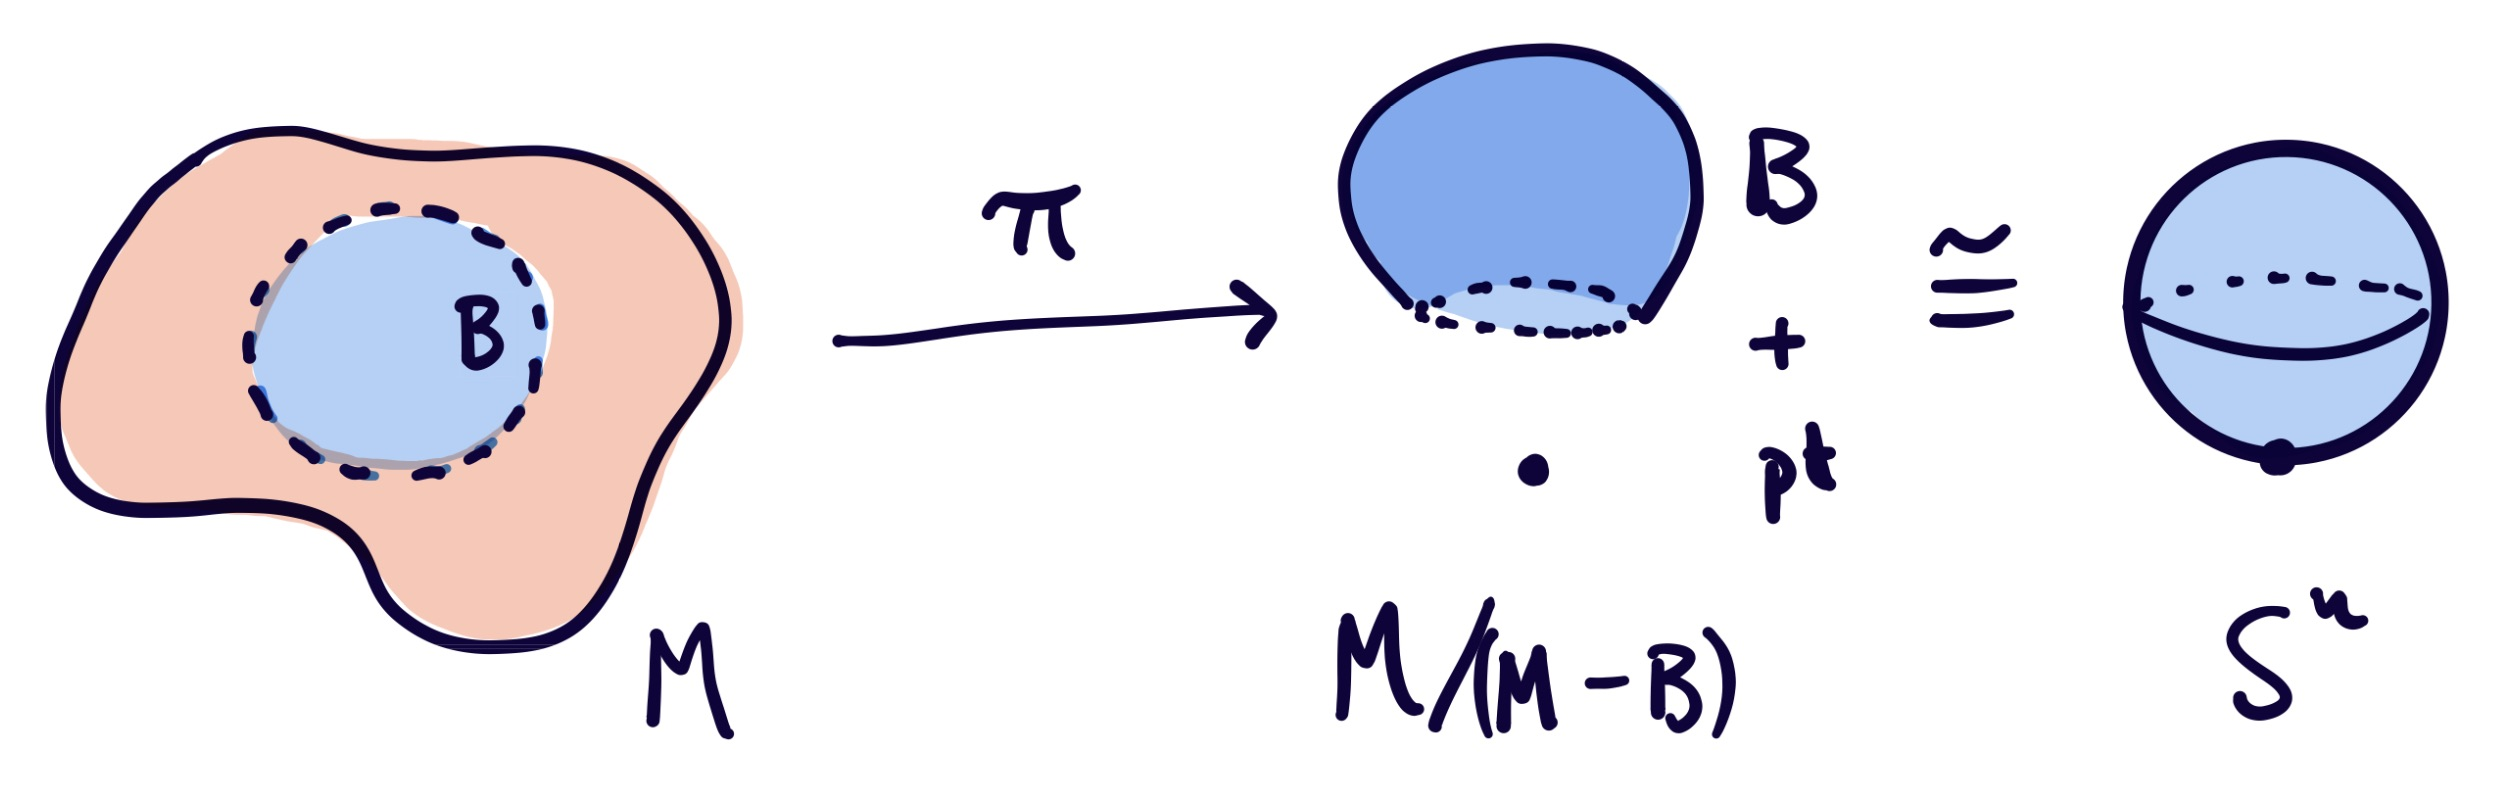
\includegraphics[width=12cm]{figures/hwk11-fig3.png}
      \captionof{figure}{The quotient $M/(M-B)$}
      \label{fig:prob17-3}
    \end{center}
  \end{prf}

  \prob[\textsc{Exercise 8.}] For a map $f:M\to N$ between connected closed orientable $n$-manifolds, suppose there is a ball $B \subseteq N$ such that $f^{-1}(B)$ is the disjoint union of balls $B_i$ each mapped homeomorphically by $f$ onto $B$. Show the degree of $f$ is $\sum_i \epsilon_i$ where $\epsilon_i$ is $+1$ or $-1$ according to whether $f:B_i\to B$ preserves or reverses local orientations induced from given fundamental classes $[M]$ and $[N]$.
  \begin{prf}
    Note first that because $M$ and $N$ are both closed connected manifolds, the inverse image $f^{-1}(B)$ has finitely many connected components. This means that we can choose a finite index set $I = \{1,...,m\}$ such that $\bigcup_{i=1}^m B_i = f^{-1}(B)$, which is good, as otherwise the sum $\sum_i \epsilon_i$ wouldn't be defined.

    Choose some $x \in B$ and denote by $x_i \in B_i$ the preimage of $x$ under $f|_{B_i}$. Consider the commutative diagram
    \begin{center}
      \begin{tikzcd}
        H_n(M) \arrow[r] \arrow[d,"f_*"]& H_n(M,\{x_i\}_{i\in I}) \arrow[d,"f_*"]\arrow[r,"\cong"]& \bigoplus_{i\in I} H_n(B_i,\{x_i\}) \arrow[d,"f_*"] \\
        H_n(N) \arrow[r]& H_n(N,\{x\}) \arrow[r,"\cong"]& H_n(B,\{x\})
      \end{tikzcd}
    \end{center}
    The leftmost horizontal maps are induced by inclusion and the rightmost horizontal isomorphisms come from the excision $M - \bigcup_{i\in I}\{B_i\}$ and $N - B$. Denote by $\mu_{x_i} \in H_n(B_i,\{x_i\})$ and $\mu_{x} \in H_n(B,\{x\})$ the generators corresponding to the fundamental classes $[M]$ and $[N]$. Under the composition of the top row of maps $[M]$ is sent to $(\mu_{x_1},...,\mu_{x_m}) \in \bigoplus_{i=1}^m H_n(B_i,\{x_i\})$, and this is mapped to $\sum_{i=1}^m \epsilon_i \mu_x$ by $f_*$ due to our assumption on $f|_{B_i}:B_i \to B$. Traversing the diagram another way, we see that $[M]$ is sent to $\deg(f)[N]$ by $f_*$, and this is mapped to $\deg(f)\mu_x$ by the composition of the bottom row maps. Commutativity of this diagram means that $\deg(f)\mu_x = \sum_{i=1}^m \epsilon_i \mu_x$, and dividing out by $\mu_x$ gives us the desired result.
  \end{prf}
\end{homework}
\end{document}
